\usetikzlibrary{arrows.meta}
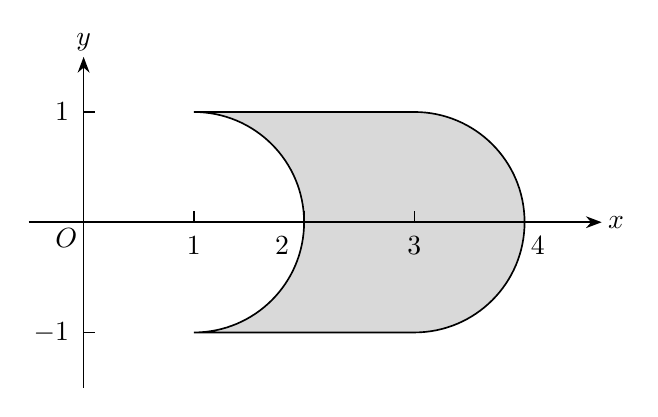
\begin{tikzpicture}[x=1.4cm,y=1.4cm,line width=.6pt,font=\normalsize,>=Stealth]
  \coordinate (C1) at (1,0);
  \coordinate (C3) at (3,0);
  \coordinate (P11) at (1,1);
  \coordinate (P31) at (3,1);
  \coordinate (P1m) at (1,-1);
  \coordinate (P3m) at (3,-1);
  \fill[black!15] (P11)--(P31) arc[start angle=90,end angle=-90,radius=1] -- (P1m) arc[start angle=-90,end angle=90,radius=1] -- cycle;
  \draw (P11)--(P31) arc[start angle=90,end angle=-90,radius=1] -- (P1m) arc[start angle=-90,end angle=90,radius=1] -- cycle;
  \draw[->] (-0.5,0) -- (4.7,0) node[right,inner sep=2pt] {$x$};
  \draw[->] (0,-1.5) -- (0,1.5) node[above,inner sep=2pt] {$y$};
  \node[below left,inner sep=2pt] at (0,0) {$O$};
  \foreach \t in {1,2,3,4}{\draw (\t,0)--(\t,0.1);}
  \node[below,inner sep=2pt,yshift=-3pt] at (1,0) {$1$};
  \node[below,inner sep=2pt,yshift=-3pt] at (1.8,0) {$2$};
  \node[below,inner sep=2pt,yshift=-3pt] at (3,0) {$3$};
  \node[below,inner sep=2pt,yshift=-3pt] at (4.12,0) {$4$};
  \foreach \t in {1,-1}{\draw (0,\t)--(0.1,\t); \node[left,inner sep=2pt,xshift=-3pt] at (0,\t) {$\t$};}
\end{tikzpicture}
